Detta projekt ämnat till att utveckla en Raviolimaskin. Ravioli är en traditionell italiensk maträtt bestående av runda eller kvadratiska pastadeg med fyllning~\cite{engproc}. Fyllningen kan bestå av till exempel köttfärs, skinka och ost. Raviolin serveras ofta i en tomatsås eller köttfärssås. Vegetarisk ravioli kan exempelvis fyllas med purjolök eller spenat.

Att laga Ravioli hemma manuellt har varit jobbigt och tidskrävande. Det finns olika typer av Raviolimaskiner på marknaden just nu som hjälper med Raviolis ifyllnings process. 

Den enklaste typen av Raviolimaskin(Ravioliplatta) visas på figue ~\ref{ravioliplatta}. Den underlättar processen, men ifyllning av Raviolin görs manuellt som medför att det tar tid och använda det.

 
	\begin{figure}[h]
		\begin{center}
			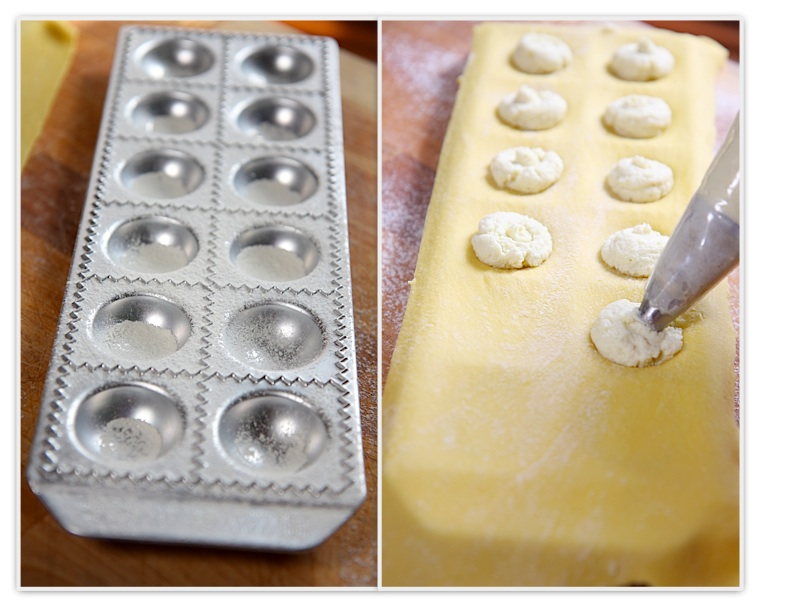
\includegraphics[scale=0.5]{images/raviolimoldwithfilling.jpg}
			\caption{Ravioliplatta för manuell ifyllning}
			\label{ravioliplatta}	
		\end{center}
	\end{figure}
En annan typ av maskin som illustreras på figur ~\ref{pastamaskin}, är väldigt stor och priset är högt som medför att de inte kan användas av hushåll.

Idén bakom detta projekt baseras på behovet av en Raviolimaskin hemma. Tanken är att utveckla en liten och relativ billig Raviolimaskin som kan vara användbar hemma.
 		\begin{figure}[h]
 			\begin{center}
 				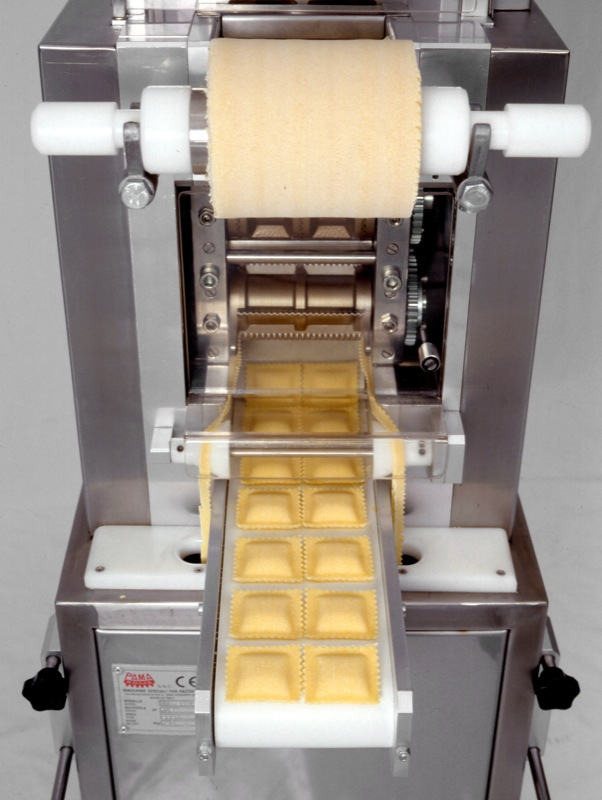
\includegraphics[scale=3]{images/pastamachine.jpg}
 				\caption{Industriell Pasta-/Raviolimaskin}
 				\label{pastamaskin}	
 			\end{center}
 		\end{figure} 